%4 結果と考察

\section{結果と考察}

\begin{figure}[t]
  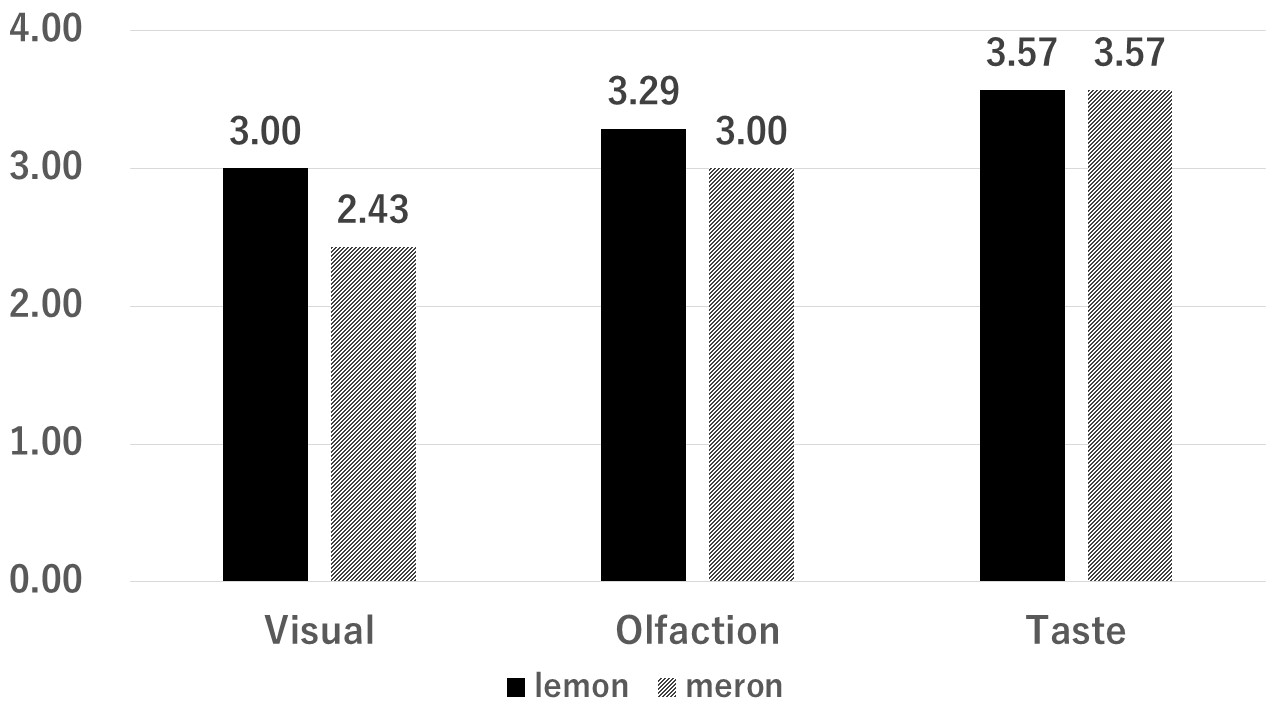
\includegraphics[width = 1.0\columnwidth]{figs/data.jpg}
  \caption{アンケートの平均スコア}
  \label{data}
\end{figure}
実験の結果を図\ref{data}に示す.


LEDで色を付けたかき氷の見た目における評価は,レモン味だと感じた平均スコアは3.00点,メロン味は2.43点であった.
これは前回の研究に引き続き,黄色がレモンの味であることを自然と印象付けている傾向にあることを示している.メロン味は半分を超えているが,印象としてはあまり良くなく,言われてみればわかるというものだった.
その一方で,「LEDによる色付けが,光っている印象が強く,色の違いが頭に入ってこなかった」という意見があった.このことから光量の強さも意識する必要がある.


嗅覚面における評価は,レモン味だと判断したのは3.29点,メロン味は3.00点であった.
どちらも評価としては高いが,意見の中で大きく違いが出た.レモン味は高い割合ではっきりとわかると答える一方で,メロン味は言われてみればという意見が多かった.自由記述にも,「あまり嗅いだことがない」,「ニオイがわかりづらい」といった記載があった.これは,メロンの香りを嗅ぎ慣れていないという体験の少なさが大きな原因となったと考えている.レモンのような柑橘系の香りは,食体験に限らず,消臭剤や芳香剤と言った身近なところにも溢れている.その一方でメロンの香りは体験することが少ないことから想起することができなかったと考えられる.


かき氷の味の感じ方の評価は,レモン味,メロン味共に3.57点と,その味を感じているという評価が多い結果となった.
レモン味は「一瞬レモンと感じたが,スプーンを離したとたんにすぐに甘い感じになった.レモンが打ち消された感覚だった」という意見から,以前の研究と同様に,一瞬の味を想起させるという目的では有効だが,しっかりと味を感じさせるという目的であれば違う手法が必要であると考える.
メロン味のほうでは.見た目と香りの評価が低いにもかかわらずメロン味の評価は高いものとなっている.
意見の中には「レモンよりもそれっぽかった」などといった,レモンに比べてポジティブなものが多かった.
その中において,メロン味のほうで,「後味がメロンの味がした」という意見を得られた.レモンとは逆で消えるのではなく残ったというのはとても興味深いものだった.甘い後味がメロンと類似するからではないかと考察する.

他にも「レモンの香りが強い」という記述が多く,ニオイの強さの制御に関しても考えていく必要がある.
